\documentclass[10pt]{article}
\usepackage[letterpaper,margin=1in]{geometry}
\usepackage[T1]{fontenc}
\usepackage{mathptmx}
\usepackage{microtype}
\usepackage{amsmath,amssymb}
\usepackage{booktabs}
\usepackage{graphicx}
\usepackage{xcolor}
\usepackage{algorithm}
\usepackage{algpseudocode}
\usepackage{tikz}
\usetikzlibrary{arrows.meta,positioning,decorations.pathreplacing}
\usepackage[numbers,sort&compress]{natbib}
\usepackage{xurl}
\usepackage[colorlinks=true,linkcolor=blue!50!black,citecolor=blue!50!black,urlcolor=blue!50!black]{hyperref}
\usepackage[capitalise]{cleveref}
\hypersetup{pdftitle={Less Budget, More Memory: Diagnosing and Mitigating Non-Monotonic Activation Memory in PyTorch's Memory-Budget Partitioner},pdfauthor={Siddharth Ajith}}

\newcommand{\code}[1]{\texttt{#1}}
\setlength{\emergencystretch}{3em}

\title{Less Budget, More Memory:\\ Diagnosing and Mitigating Non-Monotonic Activation Memory\\
in PyTorch's Memory-Budget Partitioner}
\author{Siddharth Ajith\\
Independent Researcher\\
\texttt{siddharthajith07@gmail.com}}
\date{October 2026}

\begin{document}
\maketitle

\begin{abstract}
\code{torch.compile} exposes an \code{activation\_memory\_budget} knob that trades recomputation for memory during training.
We show that the peak memory it produces is not monotone in the knob: on a 32-layer Llama-style model compiled with
Inductor, a budget of 0.05 uses 2.5$\times$ the peak memory of a budget of 0.13 (904 vs.\ 363\,MB), and a BERT model
shows the same non-monotonicity below budget 0.05.
We trace this to two limitations of AOTAutograd's min-cut partitioning pipeline. In the first (\emph{selection}), the
FLOP-maximizing knapsack that decides what to save spends small budgets on attention outputs, leaving the residual stream to
be recomputed. In the second (\emph{lifetime}), each recomputed value is defined once in the emitted backward graph, at its first backward use, and
held until its last.
Inductor's own memory estimator ranks all 14 plans we test in the same order as the measured peak (0.7\% median error);
the partitioner's in-tree evaluator does not.
We then evaluate a post-partition, use-site rematerialization pass in the style of XLA's, which recomputes cheap values
again near their late uses and leaves the saved set unchanged. At the same budget it reduces Llama's Inductor peak by
17--28\% at no measurable step-time cost, removing about half of the excess; a variant that also duplicates matrix
multiplies goes 7.5--20\% below the best stock budget on a dense grid of budgets, for 6--18\% more step time, and makes
the budget curve monotone over the budgets we tested (0.05--0.30). On BERT the excess is held dropout masks, which the pass does not
regenerate because it never duplicates random operations, so its effect there is small (0--3\%). Gradients of the rematerialization pass are checked against eager execution (Llama, every budget) or an unbudgeted run (BERT).
We also reproduce a known bug in which recomputed dropout silently corrupts gradients under a memory budget, measure
the memory cost of its proposed fix, and find that, with that fix applied, the partitioner can trigger a second,
CUDA-specific random-number bug in Inductor (PyTorch issue \#198333). All results come from one consumer GPU, two small models and fp32.
\end{abstract}

%=====================================================================
\section{Introduction}
\label{sec:intro}

Activation checkpointing trades compute for memory: instead of storing every intermediate activation for the backward
pass, some are recomputed from saved values~\citep{chen2016sublinear}.
PyTorch~2's compiler stack~\citep{ansel2024pytorch2} automates this choice.
AOTAutograd traces a joint forward--backward graph, and its min-cut partitioner decides which values the forward pass
saves. A single scalar, \code{torch.\_functorch.config.activation\_memory\_budget}~$\in[0,1]$, lets users
interpolate between the default plan (budget~1) and maximal recomputation (budget~0)~\citep{pytorchblog2025}.
Internally the partitioner solves a 0/1 knapsack: candidate values are items, their size is the weight and their estimated
recomputation runtime is the value~\citep{torchpartitioners,maczan2026knapsack}.
The budget is defined in terms of saved-activation bytes, not peak memory, so nothing promises that peak memory falls
with it; the partitioner's design note states that it ignores memory usage within each graph~\citep{he2022mincut}. Still, a user lowering the budget expects it to.

\Cref{fig:curve} shows that it need not: for a 32-layer Llama-style model the measured peak \emph{rises} from 384\,MB at
budget~0.15 to 904\,MB at budget~0.05 under Inductor (dashed gray).
The author reported this as PyTorch issue \#197838~\citep{issue197838}, and another user has since reproduced a
non-monotone curve on a GPT-style model on different hardware~\citep{lonewolf2026gist}.
This report explains why it happens and evaluates ways to mitigate it.

\begin{figure}[t]
\centering
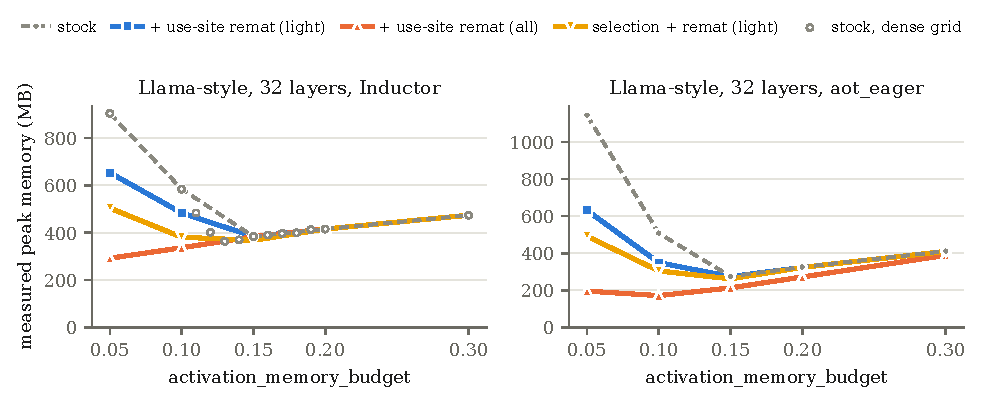
\includegraphics[width=\linewidth]{figs/fig_curve.pdf}
\caption{Measured peak allocated memory of one training step versus \code{activation\_memory\_budget}.
Stock PyTorch (dashed; hollow markers: a denser stock-only grid) is non-monotone: lowering the budget below 0.13
\emph{increases} peak memory.
Light use-site rematerialization (\cref{sec:remat}) removes about half of the excess under Inductor without changing what
is saved; its all-ops variant makes the Inductor curve monotone over the tested budgets (0.05--0.30). Where the curves coincide, the pass
changes nothing. The \code{aot\_eager} panel is a partitioner-only
ablation (\cref{sec:setup}). Numbers in \cref{tab:main}.}
\label{fig:curve}
\end{figure}

\paragraph{Contributions.}
\begin{enumerate}
\item \textbf{Diagnosis} (\cref{sec:diagnosis}). We decompose the anomaly into a selection limitation and a lifetime
limitation, with interventions under Inductor: forcing MLP outputs into the saved set lowers the low-budget peak
monotonically (904$\to$671\,MB), and splitting recomputed lifetimes with the saved set held fixed removes about half of
the excess. A sweep of sequence length and MLP size shows the selection limitation appearing only where the knapsack
values attention outputs above MLP outputs, and the lifetime limitation persisting below that point.
\item \textbf{Peak prediction} (\cref{sec:oracle}). Inductor's \code{memory.py} estimator ranks 14 plans exactly
(Spearman 1.000, 0.7\% median error). A static liveness walk over the partitioner's emitted graphs is accurate (0.4\%)
when the backend executes them as emitted, but under Inductor it only nearly preserves the ranking ($\rho=0.995$). A structural proxy we had proposed
(``closure'') and the in-tree \code{KnapsackEvaluator} do not track the peak.
\item \textbf{Use-site rematerialization for AOTAutograd} (\cref{sec:remat,sec:eval}). A post-partition pass that
recomputes a value again near its late use, as XLA's rematerialization pass does~\citep{xlaremat}. It preserves the
saved set exactly. On Llama it removes about half of the excess at the same budget, and its all-ops variant goes below
the best stock budget; on BERT, whose excess is held dropout masks, it has little effect because it never duplicates
random operations.
\item \textbf{Measurement practice} (\cref{sec:correctness}). Gradient checks that caught two pitfalls of our own
benchmark (a loss that is zero by construction, and dropout state), with controls that show the checks can fail.
\item \textbf{A correctness side finding} (\cref{sec:rng}). We independently reproduce PyTorch issue \#190758:
recomputed dropout under a memory budget silently corrupts gradients. We measure what its proposed fix costs: nothing
measurable under Inductor, 2.3--3$\times$ peak memory on a backend without its own memory planning.
\end{enumerate}
We also evaluate a liveness-aware knapsack solver as a secondary, selection-side mitigation (\cref{sec:solver}).
Schedule-aware rematerialization is not a new idea: it is central to Checkmate~\citep{jain2020checkmate},
Moccasin~\citep{bartan2023moccasin}, DTR~\citep{kirisame2021dtr}, the algorithms of \citet{kumar2019efficient}, and XLA's
rematerialization pass~\citep{xlaremat}. Our contribution is to show where PyTorch's production partitioner departs from
it, and what bringing that idea to AOTAutograd buys and costs when measured.

\paragraph{Scope.} All measurements use one consumer GPU (GTX~1650, 4\,GB), fp32, and two small model families, without
an optimizer step. We make no claims about scale, bf16, data-center GPUs or optimality (\cref{sec:limits}).

%=====================================================================
\section{Background: how the memory budget is implemented}
\label{sec:background}

AOTAutograd traces the forward and backward passes into one \emph{joint graph}.
\code{min\_cut\_\allowbreak rematerialization\_\allowbreak partition} splits it into a forward module and a backward module: it chooses a set of
forward values to \emph{save}, and every other forward value the backward needs is recomputed inside the backward module.
The split~\citep{he2022mincut,he2023fusionaware,torchpartitioners} is a minimum cut on a flow graph whose capacities are tensor sizes scaled up with distance from the backward
(and doubled for values that are not otherwise materialized), so the cut prefers saving small values close to the
backward. Some nodes are \emph{banned} from recomputation, including compute-intensive ops (matrix multiply, attention),
reductions whose output is more than 4$\times$ smaller than their inputs, and the random ops \code{native\_dropout},
\code{rand\_like} and \code{randn\_like} (a distance-based ban also exists but cannot trigger with the default
\code{max\_dist\_from\_bw}).

When $0<\text{budget}<1$ and the more aggressive default cuts do not already fit the budget,
\code{choose\_saved\_\allowbreak values\_set} does the following (at budget~0 it simply saves the inputs):
\begin{enumerate}
\item Run the min-cut with aggressive options; the nodes still banned (excluding those that alias inputs or are marked
must-save) are the knapsack \emph{candidates}.
\item Solve a 0/1 knapsack over the candidates. Weight = normalized size; value = estimated recomputation runtime (FLOPs by
default). Weights are normalized by the gap between the saved bytes of the minimal and the default plan, and the
capacity is the budget. The capacity constrains only the candidates' bytes, not the inputs or the other values the second
min-cut saves, so the saved bytes are not guaranteed to move linearly with the budget.
\item Candidates the knapsack does not select are added to \code{dont\_ban}, which lifts their ban.
\item Run the min-cut again with \code{dont\_ban}. Its result is the saved set.
\end{enumerate}
Two details matter for what follows. First, only banned nodes are candidates: pointwise ops such as \code{silu},
\code{mul} and \code{add} are never items, so the knapsack cannot see what they cost. Among the candidates, every op
without a registered FLOP formula (reductions such as the RMSNorm \code{mean} or \code{var\_mean}, dropout, embedding) is
valued at 1~FLOP, so in practice only matrix multiplies and attention carry value. Second, after partitioning,
\code{reordering\_to\_mimic\allowbreak\_autograd\_engine} orders the backward module. It inserts each recomputed forward subgraph
immediately before its \emph{first} backward consumer, and each forward value is recomputed at most once.
The tensor then lives until its \emph{last} consumer. (Inductor may still inline a cheap pointwise value into several
consumers instead of materializing it once.)
Under Inductor, the backward module is further fused, scheduled and memory-planned (including Inductor's own
\code{reorder\_for\_peak\_memory}); under \code{aot\_eager} it runs as written.

%=====================================================================
\section{Diagnosis}
\label{sec:diagnosis}

\subsection{Setup}
\label{sec:setup}
We use two Hugging Face \code{transformers} models with random weights and synthetic token inputs of shape
$2\times1024$ (batch 2, sequence 1024, vocabulary 1000).
\emph{Llama}: \code{LlamaConfig} with 32 layers, hidden size 256, MLP size 688 (SwiGLU), 8 heads, RMSNorm, SDPA attention,
no dropout.
\emph{BERT}: \code{BertConfig} with 32 layers, hidden size 192, intermediate size 768 (GELU), 3 heads, and dropout 0.1 on
attention probabilities and hidden states.
All runs: NVIDIA GTX~1650 (4\,GB) under WSL2, PyTorch 2.14.0+cu130, Python 3.12, fp32.
A training step is one forward and one backward pass (no optimizer step). Peak memory is
\code{torch.cuda.max\_memory\_allocated} during the step minus memory resident before it, which already holds the
parameters, their gradients and the inputs; it is the median of 3 steps. MB denotes $10^6$ bytes.
Peaks are deterministic within a process; across processes the same plan's peak varied by at most 1.5\,MB (0.3\%).
Step time is the median of 20 iterations timed with CUDA events after warm-up. Each case re-runs stock at the end
(drift at most 0.9\% in reported cases); across separate sessions the same stock configuration varied by up to 0.7\% on
Llama and 2.7\% on BERT, so step-time differences of about 1\% (Llama) or 2--3\% (BERT) are not meaningful.

\paragraph{Backends.} Inductor, the default \code{torch.compile} backend, is our primary setting. We also report
\code{aot\_eager}, which executes the partitioner's emitted graphs exactly as written, without fusion or rescheduling.
We use it as a \emph{partitioner-only ablation}: it removes Inductor's decompositions, joint-graph passes, fusion and
scheduling, so the partitioner sees a somewhat different joint graph (for example, 26 rather than 25 attention outputs
saved at budget 0.05), and it stands in for backends without their own memory planning. It is not a deployment configuration.

\subsection{The stock curve}
\label{sec:curve}
Under Inductor the Llama peak is 904, 584, 384, 415 and 474\,MB at budgets 0.05, 0.10, 0.15, 0.20 and 0.30
(\code{aot\_eager}: 1145, 508, 275, 325, 411\,MB; \cref{fig:curve}).
A denser stock-only grid of 18 budgets puts the minimum at 0.13 (363\,MB); the peak is 1142\,MB at budget~0 and
1110\,MB at budget~1. Above 0.13 the rise is expected: a larger budget saves more activations. Below 0.13 the rise is
the anomaly. BERT (with the dropout fix of \cref{sec:rng}) has its minimum at the lowest budget of \cref{tab:main}, 0.05
(475\,MB), and rises below it: 609, 829 and 2071\,MB at budgets 0.03, 0.02 and 0.01.

\subsection{Predicting the peak of a plan}
\label{sec:oracle}
Before changing the partitioner we need to predict what a plan costs. We evaluate predictors on 14 Llama plans per
backend (natural budgets 0.05--0.35, plans with MLP outputs forced into or out of the saved set, and the reordering
ablation below) plus 3 BERT plans (\cref{fig:oracle}).

Under Inductor, \code{torch/\_inductor/memory.py} estimates the peak of the order its scheduler chooses. Over the
14 Llama plans its estimate has Spearman $\rho=1.000$ with the measured peak, 0.7\% median and 1.5\% maximum error; on
BERT it over-predicts by 8--11\% but ranks the three plans correctly.
A static liveness walk over the partitioner's emitted forward and backward graphs (allocate each non-view output at its
definition, free it after its last use, treat saved activations as live when the backward starts) ranks the same Llama
plans almost as well ($\rho=0.995$) but is far off in absolute terms under Inductor (19\% median, 40\% maximum error),
because Inductor fuses and reschedules.
When the backend executes the emitted graphs as written (\code{aot\_eager}), the same walk is accurate: $\rho=0.999$ with
0.4\% median and 1.5\% maximum error over the 14 Llama plans; on BERT it is low by a near-constant 29--31\,MB, which
preserves ranking. Our prototypes use this walk as their oracle, also under Inductor, so under Inductor they rely only
on its near rank-correctness.

Two quantities one might use instead do not track the peak (\code{aot\_eager}, 14 Llama plans). A ``closure'' metric (the
number of unsaved candidate predecessors of each candidate, which we had earlier proposed on the issue) reaches only
$\rho=0.56$; it depends only on the saved set, so it cannot see the schedule, and it is unchanged by the reordering
ablation below while the peak changes 5.2$\times$. The in-tree \code{KnapsackEvaluator(account\_for\_backward\_pass=True)}
reaches $\rho=-0.13$. By construction it simulates only the knapsack candidates (no pointwise recomputation, no second
min-cut, no reordering) and takes the knapsack's choice as input; we did not test whether this explains its poor ranking.

\begin{figure}[t]
\centering
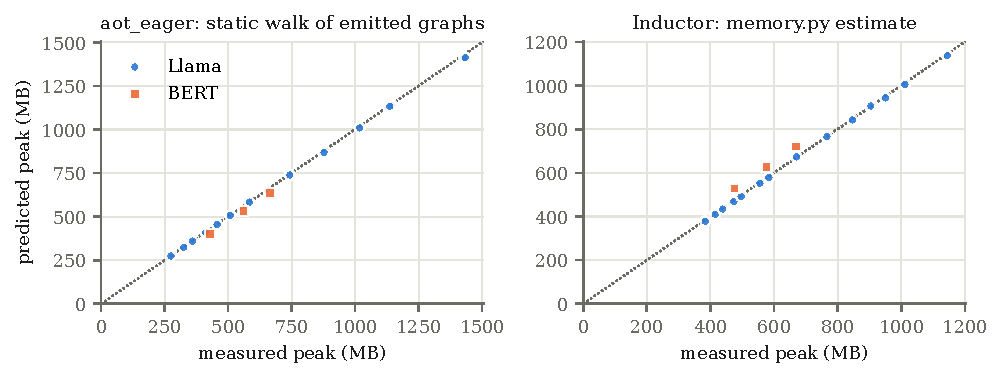
\includegraphics[width=\linewidth]{figs/fig_oracle.pdf}
\caption{Predicted versus measured peak for the 14 Llama plans (natural budgets 0.05--0.35, MLP outputs forced in or
out, reordering ablation) and 3 BERT plans (budgets 0.05--0.15, before the dropout fix of \cref{sec:rng}).
Left: static walk of the emitted graphs under \code{aot\_eager}. Right: Inductor's own \code{memory.py} estimate.
Dotted: $y=x$.}
\label{fig:oracle}
\end{figure}

\subsection{The selection limitation}
At budget 0.05 the knapsack fills the budget with attention outputs (\code{\_scaled\_dot\_product\allowbreak
\_efficient\_attention}: 25 under Inductor, 26 under \code{aot\_eager}) and saves \emph{no} MLP output. For the knapsack's
objective this is right. The partitioner's FLOP estimate charges about $4S$ FLOPs to recompute one attention output
element (causal masking is not discounted) and $2I$ for one \code{down\_proj} output element, so with sequence length
$S=1024$ and MLP size $I=688$ attention outputs are worth $2S/I\approx3$ times as much per byte. (Selective recomputation in large transformers makes the opposite choice, saving linear-layer outputs and recomputing
the attention core~\citep{korthikanti2023reducing}.) But in a pre-norm residual network the residual stream is a running sum of every layer's
\code{o\_proj} and \code{down\_proj} outputs. If those are not saved, recomputing the input of the first backward
operation requires recomputing the residual stream through all uncut layers, including their MLP internals.

The effect is causal. Under Inductor, forcing $k$ MLP outputs into the saved set at budget 0.05 lowers the peak
monotonically: 846, 766 and 671\,MB for $k=8,16,24$ (stock: 904\,MB). Conversely, forcing MLP outputs \emph{out} at
budget 0.15 raises the peak from 384 to 950\,MB. (\code{aot\_eager}: 1018, 878, 743 vs.\ 1145\,MB; 275 to 1136\,MB.)

This limitation depends on the regime. The ratio $2S/I$ exceeds 1 only when the sequence is long relative to the MLP
size. For our models it is about 3. We tested the regime directly by varying $S$ at $I=688$ and $I$ at $S=1024$ on the same
32-layer model, under Inductor on the GPU (\cref{tab:regime}). The knapsack's choice flips between ratios 0.74 and 1.49 (we tested
none in between), in both sweeps: at $2S/I=0.74$ the smallest budget saves only MLP outputs, and at every ratio above 1 only attention
outputs. Above 1, budget 0.05 uses 1.8--3.0$\times$ the peak of the best budget, and all-ops use-site rematerialization
(\cref{sec:remat}) goes 10--35\% below that best budget. At 0.74, budget 0.05 uses 1.0--1.4$\times$ the best peak and
rematerialization only matches it. The curve still rises at budget 0.02 even then (2.1$\times$), so non-monotonicity does not
need the selection limitation. A CPU run of the same sweep with the exact static oracle (\code{aot\_eager}, every budget
scored with the production knapsack solver) agrees. Stock PyTorch~2.14 neither lists the CPU attention op as compute-intensive
nor gives it a FLOP formula, so on CPU attention would never be a candidate; for this run we add both, copying the CUDA
kernels' formula. There, the knapsack's value per byte of attention outputs relative to MLP
outputs tracks $2S/I$ (0.72--5.77 against 0.74--5.95), and at $2S/I=0.74$ all-ops rematerialization brings budget 0.02 to
or below the best stock budget without changing the saved set, so the rise that remains there is the lifetime limitation.
For a model with $I=14336$, as in 8B-parameter Llama-family models, the ratio passes 1 near $S\approx7000$; we have not
tested at that scale.

\begin{table}[t]
\centering
\caption{Regime sweep under Inductor (GTX~1650; 32 layers, hidden 256, batch 2, measured peaks). Saved: attention / MLP
outputs in the knapsack's choice at budget 0.02. Excess: stock peak at that budget divided by the lowest stock peak over
budgets 0.02--0.30. All-ops: lowest peak of all-ops use-site rematerialization at budgets 0.05 and 0.10. The row
$S=1024$, $I=688$ is the configuration of \cref{tab:main}; this coarse grid has no budget 0.13, where the dense grid's
minimum is 363\,MB (\cref{sec:curve}).}
\label{tab:regime}
\small
\begin{tabular}{rrrcrrrr}
\toprule
$S$ & $I$ & $2S/I$ & saved at 0.02 & best stock (budget) & excess 0.05 & excess 0.02 & all-ops (budget) \\
\midrule
256 & 688 & 0.74 & 0 / 10 & 113.5\,MB (0.10) & 1.40$\times$ & 2.07$\times$ & 114.1\,MB (0.05) \\
1024 & 2752 & 0.74 & 0 / 25 & 489.0\,MB (0.05) & 1.00$\times$ & 2.14$\times$ & 485.4\,MB (0.05) \\
512 & 688 & 1.49 & 10 / 0 & 176.5\,MB (0.15) & 2.54$\times$ & 2.94$\times$ & 158.2\,MB (0.10) \\
1024 & 1376 & 1.49 & 15 / 0 & 398.8\,MB (0.10) & 3.04$\times$ & 3.88$\times$ & 325.1\,MB (0.05) \\
1024 & 688 & 2.98 & 10 / 0 & 383.7\,MB (0.15) & 2.36$\times$ & 2.74$\times$ & 292.3\,MB (0.05) \\
1024 & 344 & 5.95 & 7 / 0 & 385.4\,MB (0.20) & 1.78$\times$ & 2.09$\times$ & 279.7\,MB (0.10) \\
2048 & 688 & 5.95 & 10 / 0 & 913.2\,MB (0.15) & 1.99$\times$ & 2.30$\times$ & 596.7\,MB (0.05) \\
\bottomrule
\end{tabular}
\end{table}

\subsection{The lifetime limitation}
Selection alone does not explain the size of the peak. In the \code{aot\_eager} accounting at budget 0.05, tensors
recomputed in the backward account for 1069 of the 1139\,MB live at the peak (94\%). Most of them are recomputed
early, while rebuilding the
residual stream for the first backward operation, and then held until their own layer's gradient is computed, far
later. Because each value is recomputed at most once and inserted at its first use, the backward module cannot
recompute it again where it is needed later.

The schedule matters as much as the saved set. With the saved set fixed, disabling
\code{reordering\_to\_mimic\allowbreak\_autograd\_engine} raises the budget-0.15 peak from 384 to 1012\,MB under Inductor
(2.6$\times$; \code{aot\_eager}: 275 to 1434\,MB). So the order the reordering pass produces largely
determines the peak, and here it helps. By itself, though, this does not show that holding recomputed values causes the low-budget
excess. The direct evidence for that is the use-site pass of \cref{sec:remat}: with the saved set unchanged, splitting
those lifetimes removes about half of the excess under Inductor (\cref{sec:eval}).

%=====================================================================
\section{Methods}
\label{sec:methods}

\subsection{Use-site rematerialization}
\label{sec:remat}
The lifetime limitation suggests a mitigation that leaves selection alone: allow a value to be recomputed again, near
its late use. This is the idea behind XLA's \code{HloRematerialization} pass, which rematerializes values that are live
across a point where memory exceeds a limit~\citep{xlaremat}. We implement it as a pass over AOTAutograd's emitted
backward module, run after partitioning and before the backend compiler (\cref{fig:lifetime,alg:remat}).

\begin{figure}[t]
\centering
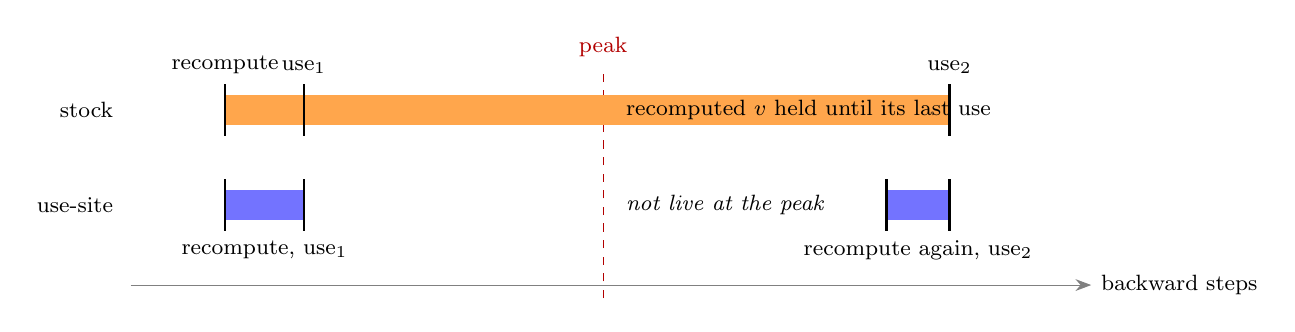
\begin{tikzpicture}[x=1cm,y=0.55cm,font=\footnotesize]
  % axis
  \draw[-{Stealth[length=2mm]},gray] (0,-0.45) -- (12.2,-0.45) node[right,black]{backward steps};
  \draw[dashed,red!70!black] (6,-0.75) -- (6,4.6) node[above]{peak};
  % stock
  \node[anchor=east] at (-0.1,3.6) {stock};
  \fill[orange!70] (1.2,3.25) rectangle (10.4,3.95);
  \node[anchor=west,inner sep=1pt] at (6.25,3.6) {recomputed $v$ held until its last use};
  \foreach \x/\l in {1.2/recompute, 2.2/use$_1$, 10.4/use$_2$}{\draw[thick] (\x,3.0) -- (\x,4.2);}
  \node[above] at (1.2,4.2) {recompute};
  \node[above] at (2.2,4.2) {use$_1$};
  \node[above] at (10.4,4.2) {use$_2$};
  % use-site
  \node[anchor=east] at (-0.1,1.4) {use-site};
  \fill[blue!55] (1.2,1.05) rectangle (2.2,1.75);
  \fill[blue!55] (9.6,1.05) rectangle (10.4,1.75);
  \foreach \x in {1.2,2.2,9.6,10.4}{\draw[thick] (\x,0.8) -- (\x,2.0);}
  \node[below] at (1.7,0.8) {recompute, use$_1$};
  \node[below] at (10.0,0.8) {recompute again, use$_2$};
  \node[anchor=west,inner sep=1pt] at (6.25,1.4) {\emph{not live at the peak}};
\end{tikzpicture}
\caption{The lifetime limitation and the use-site pass. Stock AOTAutograd recomputes a forward value $v$ once, before its first backward
use, and holds it until its last use, across the memory peak. Use-site rematerialization recomputes $v$ again just
before the late use, so it is not live at the peak. The saved set is unchanged; the cost is the duplicated (here
elementwise) work.}
\label{fig:lifetime}
\end{figure}

\begin{algorithm}[t]
\caption{Use-site rematerialization of the emitted backward module (greedy).}
\label{alg:remat}
\begin{algorithmic}[1]
\Require backward GraphModule $G$; mode $\in\{\text{light}, \text{all}\}$; cone limit $c$
\State $T \gets$ \Call{Timeline}{$G$} \Comment{static liveness walk: peak step $p$, live set at $p$, area}
\Repeat
  \For{tensors $t$ live at $p$ with a use after $p$, largest first}
    \State $u \gets$ first use of $t$ after $p$
    \State $C \gets$ backward cone of $t$, stopping at saved inputs and at values still live at $u$ for other reasons
    \If{$|C| \le c$ and every op in $C$ is allowed by mode}
      \State insert a copy of $C$ before $u$; rewire all uses of $t$ after $p$ to the copy
      \State $T' \gets$ \Call{Timeline}{$G$}
      \If{$\mathrm{peak}(T') \le \mathrm{peak}(T)$ and $(\mathrm{peak},\mathrm{area})(T') < (\mathrm{peak},\mathrm{area})(T)$}
        \State accept; remove dead code; $T \gets T'$; \textbf{break}
      \Else
        \State undo
      \EndIf
    \EndIf
  \EndFor
\Until{no change accepted, or the failure budget is exhausted}
\end{algorithmic}
\end{algorithm}

The pass never changes which values the forward saves, so saved bytes and the meaning of the budget are exactly those of
stock PyTorch. Its cost is duplicated computation. In \emph{light} mode the cone may not contain compute-intensive ops
(matrix multiplies, attention); it may contain any other non-mutating op: elementwise ops, reductions such as
\code{var\_mean} or \code{sum}, and shape and indexing ops such as \code{embedding} or \code{gather}. In \emph{all} mode matrix multiplies may be duplicated too, trading compute for
memory. Neither mode duplicates attention: every scaled-dot-product-attention op carries the
\code{nondeterministic\_seeded} tag, even without dropout, so the random-op rule below excludes it. In both modes, ops tagged \code{nondeterministic\_seeded}, Inductor's random-number primitives (such as
\code{inductor\_random}), collectives, mutating ops and ops named \code{*\_backward} are never duplicated, and cones are
limited to 12 nodes. A duplicated random op is correct only if it reproduces the forward's values, which Inductor does not
currently guarantee on CUDA (\cref{sec:correctness}), so the pass asserts that the number of random ops in the graph does
not grow.
The acceptance test uses the same static timeline as the oracle (the fx walk, also under Inductor), so every accepted
change is predicted not to raise the peak; we then measure. Because the walk only approximates Inductor's schedule, the
predicted and measured gains differ under Inductor (\cref{tab:pass}). To check the pass's decisions one by one, we
compiled and measured prefixes of its edits under Inductor (the first 1/8, 1/4, 1/2, 3/4 and all of them; Llama, budgets
0.05--0.15; the pass is deterministic, so a prefix is exactly the start of the full run). At budgets 0.05 and 0.10 the walk overstates each saving
1.3--2.2$\times$ (for the full light pass at budget 0.05 it predicts $-515$\,MB against $-251$\,MB measured), and it orders the
prefixes almost correctly ($\rho=0.94$--$1.00$ at budgets 0.05 and 0.10). In one case later edits undo part of the gain:
the all-ops pass at 0.05 reaches $-518$\,MB after half its edits and $-480$\,MB after three quarters, before ending at
$-612$\,MB. At budget 0.15 it predicts $-64$\,MB for 30 all-ops edits that change the measured peak by $-0.6$\,MB.
Inductor's own estimator (\code{memory.py}) predicts the measured change of every prefix within 6\,MB, so it is the better
acceptance test for an Inductor version of the pass.

\subsection{Liveness-aware selection (secondary)}
\label{sec:solver}
The selection limitation can also be addressed through an existing extension point: the config option
\code{activation\_memory\_budget\_solver} (in \code{torch.\_functorch.config}) accepts a custom knapsack solver. Because the
hook does not receive per-candidate runtimes or the number of forward outputs, our prototype also wraps two private
partitioner functions to obtain them, and calls the partitioner's private module-extraction function to emit plans.
It runs the stock dynamic program, emits the plan exactly as the partitioner would (the second min-cut, module extraction
and reordering), and walks it with the oracle. It then attributes the bytes of recomputed tensors live at the peak to the
nearest unsaved candidates downstream of them in the recomputation graph, raises those candidates' knapsack values, and
re-solves, for up to four rounds. A bisection on the strength of the price increase then generates a few cheaper
variants. Among all plans tried whose predicted peak is within 1\% of the best, it returns the one that keeps the most
of stock's estimated recomputation savings, and it returns the stock plan unless the predicted gain exceeds 2\%.
Every returned plan satisfies the knapsack's quantized capacity, so the budget semantics are those of stock. It used 2--7
oracle calls per graph. Choosing what to save with the schedule in view is the premise of Checkmate and
Moccasin~\citep{jain2020checkmate,bartan2023moccasin}; we include this solver as a cheap, budget-preserving instance,
not as a new idea.

%=====================================================================
\section{Evaluation}
\label{sec:eval}

\Cref{tab:main} compares each method with stock \emph{at the same budget}; \cref{tab:pareto} compares against the
\emph{best} stock budget, which is what a user who tunes the knob would get. \Cref{fig:tradeoff} plots the trade-off.

\begin{table}[t]
\centering
\small
\caption{Peak memory change versus stock at the same budget, in \%, with step-time change in parentheses. Stock peak in
MB. ``Drift'' is the step-time difference between stock and a stock re-run at the end of the case (\%).
Ind.\ = Inductor; eager = \code{aot\_eager}, a partitioner-only ablation. ``Light'' = use-site rematerialization without
matrix multiplies or attention. BERT rows are measured with the dropout fix of \cref{sec:rng} emulated. The pass never
duplicates random ops (\cref{sec:remat}); an earlier version that did is excluded (\cref{sec:samebudget}).
$^\dagger$This solver plan gives incorrect gradients, caused by PyTorch issue \#198333 (\cref{sec:correctness}); both
rows that use it are excluded from all claims.}
\label{tab:main}
\setlength{\tabcolsep}{4pt}
\begin{tabular}{llrr llll r}
\toprule
model & backend & budget & stock & remat (light) & remat (all) & selection & selection + remat (light) & drift \\
\midrule
Llama & Ind. & 0.05 & 904 & -27.7 (+0.1) & -67.7 (+12.7) & -29.0 (+5.6) & -44.3 (+5.7) & 0.2 \\
Llama & Ind. & 0.10 & 584 & -17.3 (-0.1) & -42.5 (+5.4) & -28.0 (+2.7) & -34.8 (+2.8) & 0.1 \\
Llama & Ind. & 0.15 & 384 & 0.0 (+0.1) & -0.2 (+1.0) & -4.3 (+0.1) & -4.3 (+0.1) & 0.1 \\
Llama & Ind. & 0.20 & 415 & 0.0 (+0.1) & 0.0 (+0.7) & 0.0 (+0.1) & 0.0 (-0.1) & 0.1 \\
Llama & Ind. & 0.30 & 474 & 0.0 (+0.1) & 0.0 (+0.6) & 0.0 (+0.1) & 0.0 (-0.1) & 0.1 \\
\midrule
Llama & eager & 0.05 & 1145 & -44.9 (+1.3) & -83.0 (+12.8) & -39.4 (+5.3) & -57.1 (+5.7) & 0.3 \\
Llama & eager & 0.10 & 508 & -31.3 (+0.5) & -66.4 (+4.4) & -32.3 (+1.8) & -40.1 (+1.6) & 0.1 \\
Llama & eager & 0.15 & 275 & -0.5 (+0.2) & -22.7 (+1.1) & -4.1 (-0.3) & -4.9 (-0.2) & 0.2 \\
Llama & eager & 0.20 & 325 & -0.6 (+0.3) & -16.6 (+0.9) & 0.0 (+0.1) & -0.6 (+0.1) & 0.0 \\
Llama & eager & 0.30 & 411 & -0.4 (-0.1) & -5.5 (+0.5) & 0.0 (-0.1) & -0.4 (-0.1) & 0.3 \\
\midrule
BERT & Ind. & 0.05 & 475 & -0.3 (-0.8) & +0.4 (+4.1) & -19.7 (-2.6)$^\dagger$ & -20.0 (-2.4)$^\dagger$ & 0.2 \\
BERT & Ind. & 0.10 & 575 & -0.2 (-0.1) & +6.2 (+3.9) & 0.0 (+0.0) & -0.2 (-0.2) & 0.6 \\
BERT & Ind. & 0.15 & 667 & -3.3 (-1.3) & +0.5 (+0.5) & 0.0 (-0.7) & -3.3 (-0.6) & 0.1 \\
\midrule
BERT & eager & 0.05 & 1304 & -0.2 (+0.0) & -0.2 (+0.4) & 0.0 (+0.2) & -0.2 (+0.2) & 0.7 \\
BERT & eager & 0.10 & 1432 & -0.1 (+0.0) & -0.1 (-0.2) & 0.0 (+0.1) & -0.1 (+0.0) & 0.9 \\
BERT & eager & 0.15 & 1539 & -0.1 (+0.0) & -0.1 (+0.0) & 0.0 (+0.0) & -0.1 (+0.1) & 0.2 \\
\bottomrule
\end{tabular}

\end{table}

\begin{table}[t]
\centering
\small
\caption{Under Inductor: every plan we measured whose peak is at or below the best stock plan, and not worse than
another plan in both peak and step time. $\Delta$ is relative to the best stock plan among the stock rows of
\cref{tab:main} and the dense stock grid (Llama: budget 0.13; BERT: 0.05; peaks measured in separate processes agree to
within 1.5\,MB). Step-time differences below about 1\% (Llama) and 2--3\% (BERT) are within run-to-run
variation.}
\label{tab:pareto}
\begin{tabular}{llrrrrr}
\toprule
model & method & budget & peak (MB) & step (ms) & $\Delta$peak (\%) & $\Delta$step (\%) \\
\midrule
Llama & all-ops remat & 0.05 & 292 & 914 & -19.7 & +17.7 \\
Llama & all-ops remat & 0.10 & 336 & 826 & -7.5 & +6.4 \\
Llama & stock & 0.13 & 363 & 776 & +0.0 & +0.0 \\
\midrule
BERT & light remat & 0.05 & 474 & 335 & -0.3 & -0.7 \\
BERT & stock & 0.05 & 475 & 337 & +0.0 & +0.0 \\
\bottomrule
\end{tabular}

\end{table}

\begin{figure}[t]
\centering
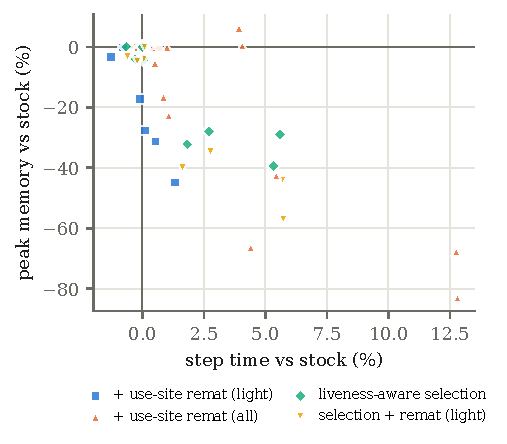
\includegraphics[width=0.55\linewidth]{figs/fig_tradeoff.pdf}
\caption{Peak memory versus step time, relative to stock at the same budget, for every case of \cref{tab:main} (plans
with incorrect gradients omitted; both backends). Points near the origin are cases where a method had no measurable effect.}
\label{fig:tradeoff}
\end{figure}

\subsection{At the same budget}
\label{sec:samebudget}
\paragraph{Light rematerialization.} Under Inductor, where the anomaly occurs (Llama at budgets 0.05 and 0.10), the pass
reduces peak memory by 27.7\% and 17.3\% with step-time changes of $+0.1\%$ and $-0.1\%$, within noise. This removes
about half of the excess over the lowest stock peak (363\,MB at budget 0.13); light mode may not duplicate matrix
multiplies, which the all-ops variant below does. Where the peak is not lifetime-driven (Llama at 0.15 and above) the
pass changes nothing measurable, and light mode is never worse than stock. On BERT under Inductor it changes the peak by
$-0.3\%$, $-0.2\%$ and $-3.3\%$ at budgets 0.05, 0.10 and 0.15. An earlier version of the pass matched random ops by
name and missed Inductor's untagged seeded primitive \code{inductor\_random}. Under Inductor it therefore regenerated
dropout masks from their saved seeds a second time, next to their late uses, where stock regenerates each mask once
before its first use. That version reduced BERT's peak by 17--21\% and passed the gradient check of
\cref{sec:correctness}, but we exclude it from all claims: whether a regenerated mask equals the forward's depends on the
dimensionality of the kernel Inductor generates for it (PyTorch issue \#198333), which the pass does not control. The gap
between the two versions shows where BERT's lifetime excess under Inductor lies: in dropout masks that the backward
regenerates once and holds until their last use. That excess becomes available to the pass once regeneration is reliable.

\paragraph{All ops.} Allowing matrix multiplies to be duplicated reduces the Llama peak under Inductor by 67.7\% at budget
0.05, for 12.7\% more step time, and makes the budget curve monotone: 292, 336, 383, 415, 474\,MB across budgets
0.05--0.30 (\cref{fig:curve}). On BERT it raises the measured peak ($+0.4\%$, $+6.2\%$ and $+0.5\%$ at budgets 0.05, 0.10 and 0.15) although the
fx walk predicts a reduction (575 to 440\,MB at 0.10, \cref{tab:pass}): under Inductor the walk can be wrong even in
sign for duplicated matrix multiplies, whose scheduling it does not model.

\paragraph{Selection.} The selection solver reduces the Llama peak under Inductor by 29.0\% and 28.0\% at budgets 0.05
and 0.10, for 5.6\% and 2.7\% more step time: unlike light rematerialization it buys memory with more expensive
recomputation, saving MLP outputs and recomputing attention instead. Combined with light rematerialization it reaches
$-$44.3\% at 0.05.

\paragraph{Partitioner-only ablation.} Under \code{aot\_eager} every effect is larger, because no scheduler reorders
around the emitted plan: light mode reaches $-$44.9\%, all-ops $-$83.0\%, and selection plus light $-$57.1\% at Llama
budget 0.05. On BERT with the dropout fix the pass has no effect there ($\le$0.2\%), because the peak is dominated by
saved dropout masks (\cref{sec:rng}).

\subsection{Against the best stock budget}
A user who sees \cref{fig:curve} would simply tune the budget. \Cref{tab:pareto} asks what each method offers beyond
the best stock plan, taken over the dense grid. On Llama, light rematerialization never goes below it (363\,MB at budget
0.13): it removes part of the anomaly but does not beat tuning the knob. The all-ops variant does, at a price: $-$7.5\%
peak for $+$6.4\% step time at budget 0.10, and $-$19.7\% for $+$17.7\% at 0.05. The selection solver's lowest plan
(367\,MB at budget 0.15) is 1\% above the best stock plan. On BERT no method we measured goes meaningfully below the best
stock plan (light rematerialization at 0.05: $-0.3\%$). On these models, all-ops rematerialization is the only method that
extends the memory floor, at an explicit compute cost.

\subsection{Compile-time overhead}
\Cref{tab:pass} lists the work done by the pass. Our prototype re-walks the whole backward after every accepted change;
in the runs of \cref{tab:main} it takes 1--48\,s per graph, and the selection solver 5--72\,s. Both are acceptable for
an opt-in prototype and not for a default; an incremental timeline would remove most of the pass's cost. Under Inductor
the pass also enlarges the graph that Inductor compiles: Llama's total compile time at budget 0.05 rises from 113\,s
(stock) to 151\,s with light and 176\,s with all-ops rematerialization (+56\%). The cost is paid once per compiled graph:
the largest increase (63\,s) is about 0.8\% of 10,000 training steps at that configuration's 0.81\,s step, and BERT's
longest Inductor pass (27\,s) about 0.8\% at 0.34\,s.

\begin{table}[t]
\centering
\small
\caption{Work done by the use-site pass at the low budgets: predicted backward peak before and after (MB, static walk),
accepted rematerializations, added work per step in units of $10^9$ (a normalized proxy, not FLOPs: exact FLOPs for matrix
multiplies, one unit per output element for every other op; neither mode duplicates attention, \cref{sec:remat}; step
time in \cref{tab:main} is the measured cost), and pass time (s, Python, unoptimized).}
\label{tab:pass}
\begin{tabular}{llrlrrrr}
\toprule
model & backend & budget & mode & predicted peak & accepted & added work & time \\
\midrule
Llama & Ind. & 0.05 & light & 1150 $\to$ 634 & 180 & 0.54 & 29 \\
Llama & Ind. & 0.05 & all & 1150 $\to$ 200 & 282 & 149.70 & 46 \\
Llama & eager & 0.05 & light & 1139 $\to$ 628 & 179 & 0.28 & 30 \\
Llama & eager & 0.05 & all & 1139 $\to$ 193 & 280 & 149.16 & 48 \\
Llama & Ind. & 0.10 & light & 586 $\to$ 379 & 69 & 0.22 & 15 \\
Llama & Ind. & 0.10 & all & 586 $\to$ 171 & 115 & 63.55 & 24 \\
Llama & eager & 0.10 & light & 506 $\to$ 345 & 54 & 0.09 & 14 \\
Llama & eager & 0.10 & all & 506 $\to$ 167 & 98 & 51.95 & 22 \\
BERT & Ind. & 0.05 & light & 444 $\to$ 311 & 79 & 0.14 & 19 \\
BERT & Ind. & 0.05 & all & 444 $\to$ 309 & 109 & 9.49 & 25 \\
BERT & Ind. & 0.10 & light & 575 $\to$ 442 & 77 & 0.12 & 20 \\
BERT & Ind. & 0.10 & all & 575 $\to$ 440 & 107 & 9.48 & 27 \\
BERT & eager & 0.05 & light & 1271 $\to$ 1269 & 3 & 0.00 & 1 \\
BERT & eager & 0.05 & all & 1271 $\to$ 1269 & 3 & 0.00 & 1 \\
BERT & eager & 0.10 & light & 1401 $\to$ 1400 & 3 & 0.00 & 1 \\
BERT & eager & 0.10 & all & 1401 $\to$ 1400 & 3 & 0.00 & 1 \\
\bottomrule
\end{tabular}

\end{table}

\subsection{Correctness}
\label{sec:correctness}
A memory optimization that changes gradients is worthless, and checking for this was subtle enough that we describe it here.
\begin{itemize}
\item \textbf{Llama} (no randomness). Against an uncompiled fp32 eager reference at budget 0.05 under Inductor, the relative
$L_2$ error of the full gradient is $3.33\times10^{-7}$ for stock, $3.34\times10^{-7}$ with light rematerialization and
$3.33\times10^{-7}$ with all-ops rematerialization (stock against a stock re-run: $1.2\times10^{-9}$); the differences
are float reassociation from different fusion. Repeating this check at every budget from 0.05 to 0.30 on both backends
gives errors of $3.30$--$3.38\times10^{-7}$ under Inductor and $1.98$--$2.04\times10^{-7}$ under \code{aot\_eager} for
stock, light and all-ops plans alike (stock against a stock re-run: at most $6.1\times10^{-9}$). The selection solver's
Llama plans were compared against stock, which they match to at most $2\times10^{-7}$.
\item \textbf{BERT.} Two pitfalls nearly misled us. First, the benchmark's training wrapper returns the sum of the final
LayerNorm output, which is zero by construction; its ``gradients'' are mostly float residue, and comparisons of them are
weak evidence. For every BERT correctness claim we therefore use a fixed random projection of the outputs as the loss.
Second, dropout makes the result depend on the random number generator, so we reseed before every step and compare
against budget 1.0, where nothing is recomputed. With dropout disabled, stock and light plans at budget 0.05 match budget
1.0 to $3.2\times10^{-7}$ and $3.1\times10^{-7}$. With dropout enabled and the fix of \cref{sec:rng} emulated, stock,
light and all-ops plans (corrected pass) match budget 1.0 to $2.3$--$3.0\times10^{-7}$ at budgets 0.05, 0.10 and 0.15;
the pass accepted 71--109 rematerializations in these plans, so the check is not vacuous, and the number of random ops in
every backward graph was unchanged (97). The earlier version of the pass (\cref{sec:samebudget}), which did duplicate
random ops, also passed this check ($2.6$--$2.8\times10^{-7}$); we do not take that as evidence that it is safe, because
on CUDA the result depends on kernel shapes that the next item shows can change. With the fix disabled, the same test reports
5.1--5.3\% errors for every plan on a smaller CPU model, so it does detect mismatched dropout masks.
\item \textbf{The selection solver on BERT under Inductor.} At budget 0.05, with dropout enabled and the fix emulated,
the solver's plan gives gradients that differ from budget 1.0 by $2.0\times10^{-2}$, while stock differs by
$2.2\times10^{-7}$ in the same run (\cref{tab:main}, $\dagger$). The backward of that plan does not depend on the global
random state (advancing it between forward and backward changes gradients by only $2\times10^{-7}$), and the \emph{same}
saved set, mapped onto the dropout-free graph (241 of 241 saved candidates mapped), gives correct gradients
($2.9\times10^{-7}$). Reverting, one class at a time, the five operator classes in which the plan differs from stock
isolates the cause: reverting only the 65 saved \code{var\_mean} nodes (LayerNorm statistics) restores correct gradients ($2.7\times10^{-7}$), while reverting any other
class leaves the error at $2.0\times10^{-2}$. In the tested configuration, the cause is PyTorch issue \#198333~\citep{issue198333}: since
PyTorch~2.13, Inductor's CUDA code generator draws random numbers with one function in one-dimensional kernels and
another in multi-dimensional (tiled or reduction) kernels, and the two give different values for the same seed and offset. When the
statistics are saved, the backward regenerates some dropout masks in one-dimensional kernels, while the forward
generated all of them in multi-dimensional ones, so those masks differ. Recording which function each kernel used is
consistent with this (the forward used only \code{tl.rand}; the backward used \code{rand4x} in 63 one-dimensional kernels),
and disabling the one-dimensional variant (we patch Inductor's private \code{TritonOverrides.\_can\_use\_4x\_random} to
return false; all else unchanged) makes the same plan correct: its gradients match budget
1.0 to $2.6\times10^{-7}$ (stock: $2.5\times10^{-7}$), with the same 381.5\,MB peak as before and no measurable change in
step time. The failure is therefore not in the solver or in our emulation of the dropout fix. We still exclude the
affected rows, which were measured with the faulty path enabled.
\end{itemize}

\paragraph{Negative results.} A variant of the selection solver that additionally forced fractions of
repeated-structure candidate classes, ranked by peak attribution, gave identical measured peaks in all six cases we
tried, at 1.4--2.2$\times$ the solver time. An earlier, broader class-forcing search found gains the repricing solver
misses (Llama \code{aot\_eager}: $-$10.2\%, $-$15.8\% and $-$5.4\% at budgets 0.15, 0.20 and 0.30), so the solver is not
close to optimal there. Finally, the default FLOP-based runtime estimate is a poor proxy for cost: for one Llama plan it
predicted keeping only 40\% of stock's recomputation savings, yet the measured step time rose by only 5\%; PyTorch's
profiling-based estimator predicted that cost within about 5\%.

%=====================================================================
\section{Side finding: randomness under memory budgets}
\label{sec:rng}
While validating BERT we found that whenever the partitioner reaches its knapsack path (or budget 0), the backward module
can recompute dropout with fresh randomness,
so its masks differ from the forward's and gradients are silently wrong. This is the open PyTorch issue
\#190758~\citep{issue190758}, which already identifies the Inductor path through \code{prims.inductor\_seeds} and
proposes saving the outputs of random ops~\citep{pr190759}; replaying the random state is an
alternative~\citep{pr191684}. We reproduced it independently and measured three things.
\begin{enumerate}
\item \textbf{Reproducers.} A stack of eight Linear--GELU--Dropout blocks on CPU has a 21.5\% gradient error under
Inductor at budget 0, confirmed by a finite-difference check; under \code{aot\_eager} gradients are 18--22\% wrong at
every budget below 1 that we tested (0.9, 0.5, 0.1, 0). On a 4-layer BERT on CPU under Inductor, advancing the global
random state between forward and backward changes the budget-0.05 gradient by 3.7\% (budget 1: $2.7\times10^{-7}$).
On the GPU BERT, the budget-0.05 gradient differs from budget 1.0 by $2.0\times10^{-2}$ with identical forward masks.
\item \textbf{The proposed fix works.} Emulating it (no op tagged \code{nondeterministic\_seeded} is recomputed) reduces
the CPU BERT error from 3.5\% to at most $4\times10^{-7}$.
\item \textbf{What the fix costs.} Under Inductor it saves only the small seeds tensor: at budgets 0.05, 0.10 and 0.15 the stock
BERT peak changes by less than the run-to-run variation across processes (at most 1.5\,MB). On a backend that executes the
emitted graph as written (\code{aot\_eager}) the fix saves full dropout masks, and the peak rises from 430 to 1304\,MB
at budget 0.05 (560 to 1432 and 665 to 1539\,MB at 0.10 and 0.15). This is quantitative input for choosing between
saving random outputs and replaying random state.
\end{enumerate}
All BERT numbers in \cref{tab:main} are measured with the fix emulated, so they describe the corrected baseline.

Memory budgets also expose a second, independent random-number bug. The wrong solver gradients of
\cref{sec:correctness} come from PyTorch issue \#198333~\citep{issue198333}, in which Inductor's CUDA code regenerates
dropout masks with a different random function when the backward kernel's dimensionality differs from the forward's.
The issue reports it through \code{torch.utils.checkpoint}; we reach it without any checkpoint API, through the
memory-budget partitioner with the proposed fix for \#190758 applied, by saving a different set of activations.

%=====================================================================
\section{Related work}
\label{sec:related}
\paragraph{Schedule-aware rematerialization.}
Checkmate formulates rematerialization jointly with the schedule as a mixed-integer program and finds optimal plans
offline~\citep{jain2020checkmate}; Moccasin reformulates it with retention intervals and constraint
programming~\citep{bartan2023moccasin}. MONeT jointly optimizes checkpointing and operator
implementations~\citep{shah2021monet}, POET adds paging for edge devices~\citep{patil2022poet}, and Rockmate combines
block dynamic programming with integer programming for PyTorch models~\citep{zhao2023rockmate}. These methods are optimal
or near-optimal but rely on offline solvers; our setting is a production compiler with seconds of compile-time budget and
an existing API contract. XLA's rematerialization pass~\citep{xlaremat} is the direct ancestor of our use-site pass, and recomputing a value near
each use instead of extending its live range is classic register-allocation rematerialization~\citep{briggs1992remat};
\citet{kumar2019efficient} give rematerialization schedules with provable guarantees for graphs of bounded treewidth.
Echo~\citep{zheng2020echo} and SuperNeurons~\citep{wang2018superneurons} recompute only cheap layers in the backward,
as our light mode does. \citet{he2023fusionaware} make AOTAutograd's min-cut fusion-aware, the partitioner we study.
\paragraph{Dynamic and allocator-aware approaches.}
DTR evicts and recomputes at runtime~\citep{kirisame2021dtr}; Coop makes this fragmentation-aware~\citep{zhang2023coop}.
A recent simulator study of DTR reports regime switching and a ``feasibility inversion'' in which training is possible at one
budget, impossible at a larger one and possible again at a larger one still~\citep{pagadala2026regime}. That
non-monotonicity has a different mechanism, in a different system, from ours.
\paragraph{Ordering and layout.} OLLA~\citep{steiner2022olla} and ROAM~\citep{shu2023roam} reduce peak memory by
optimizing operator order and tensor placement without recomputation; Inductor's \code{reorder\_for\_peak\_memory} is a
production instance. Inductor's reordering is enabled in all our Inductor runs and does not undo the anomaly.
\paragraph{PyTorch.} The memory-budget API is described in~\citep{pytorchblog2025} and its knapsack is implemented
in~\citep{torchpartitioners};
\citet{maczan2026knapsack} reduce the knapsack solver's own memory, and issue \#149258~\citep{issue149258} reports the
same residual-stream recomputation chain from the speed side. Several tools choose what to save against an absolute
per-device memory budget: PyTorch's \code{sac\_milp} formulation for selective activation
checkpointing~\citep{sacilp}, and a budget-aware keep/recompute/offload policy proposed for
torchtitan~\citep{torchtitan4636}. Such tools decide \emph{what} to save; the placement of recomputation inside the
backward is still left to the partitioner, as it is for PyTorch's tag-based rematerialization pass
(\code{remat\_using\_tags\_for\_fwd\_loss\_bwd\_graph}), which likewise recomputes each node once at its first backward use. The use-site pass is complementary to all of them.
\paragraph{Concurrent work.}
We reimplemented the greedy save-set selector of~\citet{somers2026checkpointing} from its published description and ran
it on a CPU toy model (16-layer Llama-style model, \code{aot\_eager}, exact static oracle): at matched peak it recomputes
1.3--17$\times$ fewer FLOPs than our liveness-aware solver, and use-site rematerialization lowers its final plan slightly
further (58.9$\to$58.3\,MB), consistent with selection and lifetime being separate limitations. Our reimplementation may
differ from the original, and we have not run it on our GPU setup.

%=====================================================================
\section{Limitations and future work}
\label{sec:limits}
\begin{itemize}
\item \textbf{Scale.} One 4\,GB consumer GPU, fp32, two small model families, no optimizer step. Whether the anomaly and the
gains persist at 1--8B parameters, in bf16 and on data-center GPUs is untested. The selection limitation appears only when
$2S/I>1$ (\cref{tab:regime}); that sweep varies $S$ and $I$ on the 32-layer, hidden-256 model only.
\item \textbf{End-to-end metric.} We report peak memory and step time, not the largest batch or sequence that fits.
\item \textbf{Baselines.} We compare against stock at the same and at the best budget, but not against optimal plans
(Checkmate or Moccasin on small graphs), manual checkpointing policies, or absolute-budget planners.
\item \textbf{Oracle under Inductor.} Our prototypes use the fx walk as their oracle even under Inductor, where it only nearly
preserves the ranking of plans and overstates the pass's savings 1.3--2.2$\times$ at budgets 0.05 and 0.10 (\cref{sec:remat}). Inductor's own
estimator, which predicts the effect of the pass's edits within 6\,MB, would be the better choice.
\item \textbf{Safety of the pass beyond our graphs.} Duplication is safe in the functional backward graphs we tested; graphs
with in-place mutation of storage (for example under fully sharded data parallelism) would need storage-aware checks, and
the pass's list of compute-intensive ops is matched by name.
\item \textbf{Compile time.} The prototypes add tens of seconds per graph (up to +56\% total compile time for Llama under
Inductor).
\item \textbf{Random-number regeneration.} The pass never duplicates random operations, which forgoes BERT's lifetime
gain (\cref{sec:samebudget}). Under a budget, Inductor already regenerates each dropout mask once from its saved seed;
regenerating it again near a late use relies on the same mechanism, but on CUDA it is reliable only once PyTorch issue
\#198333 is fixed. We did not test the earlier version of the pass with the affected code path disabled.
\item \textbf{PyTorch issue \#198333.} Our results use PyTorch~2.14, which has this bug. Until it is fixed, plans that
change the shape of the kernels that regenerate dropout masks can give wrong gradients on CUDA; this is what happened to
the solver on BERT (\cref{sec:correctness}). Disabling the affected code path, as we did by patching a private Inductor
function, is a workaround; we did not test the \code{align\_random\_eager} setting that the issue suggests.
\end{itemize}
The natural next steps are an incremental version of the pass that uses Inductor's estimator, combining it with a
selection policy evaluated after rematerialization, evaluation on larger models, and a discussion with PyTorch
maintainers about offering the pass behind a flag.

\section*{Reproducibility}
Scripts, per-run JSON results, logs and this paper's source are available at\\
\url{https://github.com/siddddd17/less-budget-more-memory}.
All tables and figures are generated by a script from the per-run JSON files, and every other number is in a JSON or log
file produced by the script named in the repository's README. The GPU results require a CUDA GPU to rerun; the CPU
results run on any machine.

\section*{Acknowledgments}
We thank Aiswarya for lending the laptop with the GTX~1650 GPU on which all experiments were run.

\bibliographystyle{plainnat}
\bibliography{refs}
\end{document}
